\documentclass[12pt]{article}%
\usepackage{amsfonts}
\usepackage{fancyhdr}
\usepackage{comment}
\usepackage[a4paper, top=2.5cm, bottom=2.5cm, left=2.2cm, right=2.2cm]%
{geometry}
\usepackage{times}
\usepackage{placeins}
\usepackage{amsmath}
\usepackage{changepage}
\usepackage{amssymb}
\usepackage{tikz}
\usepackage{float}
\usepackage{graphicx}%

\usepackage{listings}
\usepackage{color}

\definecolor{mygreen}{rgb}{0,0.6,0}
\definecolor{mygray}{rgb}{0.5,0.5,0.5}
\definecolor{mymauve}{rgb}{0.58,0,0.82}


\setcounter{MaxMatrixCols}{30}
\newtheorem{theorem}{Theorem}
\newtheorem{acknowledgement}[theorem]{Acknowledgement}
\newtheorem{algorithm}[theorem]{Algorithm}
\newtheorem{axiom}{Axiom}
\newtheorem{case}[theorem]{Case}
\newtheorem{claim}[theorem]{Claim}
\newtheorem{conclusion}[theorem]{Conclusion}
\newtheorem{condition}[theorem]{Condition}
\newtheorem{conjecture}[theorem]{Conjecture}
\newtheorem{corollary}[theorem]{Corollary}
\newtheorem{criterion}[theorem]{Criterion}
\newtheorem{definition}[theorem]{Definition}
\newtheorem{example}[theorem]{Example}
\newtheorem{exercise}[theorem]{Exercise}
\newtheorem{lemma}[theorem]{Lemma}
\newtheorem{notation}[theorem]{Notation}
\newtheorem{problem}[theorem]{Problem}
\newtheorem{proposition}[theorem]{Proposition}
\newtheorem{remark}[theorem]{Remark}
\newtheorem{solution}[theorem]{Solution}
\newtheorem{summary}[theorem]{Summary}
\newenvironment{proof}[1][Proof]{\textbf{#1.} }{\ \rule{0.5em}{0.5em}}

\newcommand{\Q}{\mathbb{Q}}
\newcommand{\R}{\mathbb{R}}
\newcommand{\C}{\mathbb{C}}
\newcommand{\Z}{\mathbb{Z}}

\usetikzlibrary{arrows.meta,
	quotes
}
\usetikzlibrary{automata,positioning}

\lstset{ 
	backgroundcolor=\color{white},   % choose the background color; you must add \usepackage{color} or \usepackage{xcolor}; should come as last argument
	basicstyle=\footnotesize,        % the size of the fonts that are used for the code
	breakatwhitespace=false,         % sets if automatic breaks should only happen at whitespace
	breaklines=true,                 % sets automatic line breaking
	captionpos=b,                    % sets the caption-position to bottom
	commentstyle=\color{mygreen},    % comment style
	deletekeywords={...},            % if you want to delete keywords from the given language
	escapeinside={\%*}{*)},          % if you want to add LaTeX within your code
	extendedchars=true,              % lets you use non-ASCII characters; for 8-bits encodings only, does not work with UTF-8
	frame=single,	                   % adds a frame around the code
	keepspaces=true,                 % keeps spaces in text, useful for keeping indentation of code (possibly needs columns=flexible)
	keywordstyle=\color{blue},       % keyword style
	language=C,		                 % the language of the code
	morekeywords={*,...},            % if you want to add more keywords to the set
	numbers=left,                    % where to put the line-numbers; possible values are (none, left, right)
	numbersep=5pt,                   % how far the line-numbers are from the code
	numberstyle=\tiny\color{mygray}, % the style that is used for the line-numbers
	rulecolor=\color{black},         % if not set, the frame-color may be changed on line-breaks within not-black text (e.g. comments (green here))
	showspaces=false,                % show spaces everywhere adding particular underscores; it overrides 'showstringspaces'
	showstringspaces=false,          % underline spaces within strings only
	showtabs=false,                  % show tabs within strings adding particular underscores
	stepnumber=2,                    % the step between two line-numbers. If it's 1, each line will be numbered
	stringstyle=\color{mymauve},     % string literal style
	tabsize=2,	                   % sets default tabsize to 2 spaces
	title=\lstname                   % show the filename of files included with \lstinputlisting; also try caption instead of title
}

\newcommand{\addCode}[2]{
	\lstinputlisting[caption=#2]{Code/#1.c}
}

\begin{document}

\title{Plan de gesti\'on, an\'alisis, dise\~no y memoria del proyecto}
\author{Spread Your Music}
\date{\today}
\maketitle

\tableofcontents

\newpage

%% Section 1

\section{Introducci\'on}

\subsection{Resumen}

La aplicaci\'on a desarrollar consistir\'a en un reproductor de m\'usica en \textit{streaming} inspirado en \textit{Soundcloud} y \textit{Spotify}.\\ 

Es una aplicaci\'on orientada a todo tipo de usuario, tanto a los m\'usicos que est\'an empezando su carrera en el mundo de la m\'usica como a cualquier persona aficionada a la m\'usica. Nuestra aplicaci\'on permitir\'a a los usuarios subir canciones, crear listas de reproducci\'on o escuchar canciones utilizando un reproductor propio entre otras funcionalidades. La versi\'on Android permitir\'a a los usuarios descargar las canciones para poder escucharlas sin necesidad de estar conectado a Internet. Tambi\'en incluir\'a caracter\'isticas sociales, permitiendo a los usuarios seguir a sus artistas favoritos para ver las novedades que publican o suscribirse a listas de reproducci\'on creadas por otros usuarios para enterarse de cambios en esta. El sistema tambi\'en poseer\'a integraci\'on con redes sociales, as\'i como la posibilidad de autentificaci\'on mediante cuenta de Google.\\

El usuario tendr\'a recomendaciones personalizadas para el usuario tanto basadas en su historial de reproducci\'on como en geolocalizaci\'on y facilitar\'a al usuario encontrar canciones, pudiendo buscar canciones por categor\'ias, autor, nombre, as\'i como tambi\'en mostrando canciones populares dentro de la aplicaci\'on.\\

Nuestra aplicaci\'on tendr\'a soporte web (en navegadores Chrome y Firefox) y como aplicaci\'on Android, de manera que el usuario pueda usarla en web, en el m\'ovil o en ambas ya que incorpora un sistema de sincronizaci\'on de manera que el usuario puede seguir escuchando en cualquier dispositivo la misma canci\'on justa en el momento en el que la dej\'o. \\


%% Section 2

\section{Organizaci\'on del proyecto} % Main chapter title
\subsection{Equipo}

El equipo est\'a formado por 7 estudiantes de Ingenier\'ia Inform\'atica: Jorge Aznar L\'opez, \'angel Ca\~nal Muniesa, Abel Chils Trabanco, Alicia Yasmina Albero Escudero, \'oscar Fraca Ferr\'andez, Alexandru Ioan Oarga Hategan y Jorge Pinilla L\'opez.\\

De estos, cinco poseen conocimientos sobre programaci\'on Web (\textit{Frontend}) as\'i como pr\'actica en el desarrollo del \textit{Backend} de una aplicaci\'on Web. Por otro lado, todos tienen experiencia en el dise\~no de base de datos, as\'i como experiencia con la programaci\'on sobre la plataforma Android. Adem\'as, los integrantes del grupo ya poseen experiencia trabajando juntos, lo cual facilitar\'a la comunicaci\'on entre ellos. \\

Para desarrollar esta aplicaci\'on se han creado 3 grupos y cada uno se centrar\'a en una parte del desarrollo. Un equipo se encargar\'a del
\textit{Backend}, otro de la interfaz Web (o \textit{Frontend}) y por \'ultimo otro de la aplicaci\'on Android. La asignaci\'on de los integrantes del grupo a cada una de las partes se ha realizado en base a la experiencia que posea el integrante en cuesti\'on en dicha \'area.\\

El equipo de \textit{Backend} est\'a formado por \'oscar, \'angel y Jorge Aznar. El equipo de la plataforma Android est\'a formado por Abel y Yasmina. Por \'ultimo, el equipo de \textit{Frontend} est\'a formado por Alexandru y Jorge Pinilla. \\

Para gestionar el proyecto se ha designado un coordinador general y coordinadores espec\'ificos dentro de cada \'area. El coordinador general es Abel, el coordinador de \textit{Backend} es \'angel, el de Android es Abel y el de \textit{Frontend} es Jorge Pinilla

%% Section 3

\section{Plan de gesti\'on del proyecto} % Main chapter title

\subsection{Procesos}

\subsubsection{Procesos de inicio de proyecto}

La aplicaci\'on m\'ovil funcionar\'a en dispositivos con Android 5.0, la aplicaci\'on web funcionar\'a en los navegadores Firefox y Chrome. Para realizar las pruebas de la aplicaci\'on m\'ovil se requerir\'a de un dispositivo con Android 5.0. Por otro lado, para las pruebas de la versi\'on web ser\'a necesario un ordenador con el navegador instalado (Chrome o Firefox). El sistema se funcionar\'a sobre un cl\'uster, que contar\'a con un almacenamiento bruto de 20GB. Se ha estimado este tama\~no para el cl\'uster teniendo en cuenta la arquitectura del sistema. 


\subsubsection{Procesos de ejecuci\'on y control del proyecto}

Las comunicaciones del grupo se van a realizar mediante un grupo en la aplicaci\'on de mensajer\'ia instant\'anea \textit{WhatsApp} para tratar temas y comunicaciones poco importantes y eventuales. Sin embargo, para temas que deban ser permanentes y/o deba quedar constancia de esta comunicaci\'on, se usar\'an las \textit{Issues} o incidencias de la plataforma de alojamiento de los proyectos \textit{GitHub}. En esta plataforma de alojamiento se almacenar\'a el c\'odigo fuente del sistema desarrollado y todos los documentos generados durante el desarrollo. Entre estos documentos se encuentra, por ejemplo, las actas de las reuniones con los clientes, que ser\'an redactadas por al menos un miembro del equipo durante dicha reuni\'on. De forma similar se registrar\'an las reuniones del equipo, los contenidos y las decisiones que puedan tomarse en esas reuniones.\\

En todas las actas, tanto de reuniones del equipo como reuniones con los clientes se incluir\'a al menos la fecha y hora de la reuni\'on, la duraci\'on de la reuni\'on, los miembros presentes en la reuni\'on y los temas y decisiones que se tomen en la reuni\'on.\\

Todas las semanas tienen un conjunto de tareas asociadas. Al final de cada semana, el responsable de cada proyecto revisar\'a las tareas que se han realizado esa semana y, si hay tareas que no se han cumplido, se asignar\'an autom\'aticamente para la siguiente semana, siendo estas tareas las primeras que se deber\'an hacer. Adem\'as, cada semana el responsable del subproyecto revisar\'a cuantas tareas se han realizado para la siguiente iteraci\'on  como m\'etrica de monitorizaci\'on de la desviaci\'on seg\'un el plan original. Tras esta revisi\'on el responsable del subproyecto asignar\'a las tareas de la semana a todos los miembros del equipo que puedan trabajar esa semana. \\

Durante el desarrollo del proyecto puede haber problemas y disputas entre los miembros del equipo. Para tratar de resolverlos el responsable del subproyecto ser\'a el primero en mediar entre los miembros en disputa y, si hay alguna raz\'on que haga imposible esta mediaci\'on ser\'a el resto del equipo quien deber\'a mediar. \\

\subsubsection{Procesos t\'ecnicos}
Las herramientas utilizadas tanto para desarrollo del software (construcci\'on, pruebas y despliegue) ser\'an IntelliJ Idea y Android Studio debido a que ambas dan soporte para los lenguajes de programaci\'on Java y Kotlin adem\'as de su buena integraci\'on con git, herramienta que se utilizar\'a para el control de versiones. En el caso especial del Frontend se usar\'a como herramienta WebStorm por razones similares a los anteriores.\\

Para asegurar la calidad del software, al mismo tiempo que se vaya desarrollando se ir\'an creando pruebas unitarias sobre el mismo con JUnit.\\

Siguiendo una metodolog\'ia de diseño incremental, cada dos semanas se tiene planificada la entrega interna de una versi\'on nueva del software.  Estas versiones se basa en la versi\'on anterior añadi\'endole ciertas funcionalidades.\\


\subsection{Planes}
\subsubsection{Plan de gesti\'on de configuraciones}

El c\'odigo desarrollado deber\'a seguir una serie de est\'andares, siendo los siguientes los aceptados. Para el nombrado de m\'etodos, variables, clases... se utilizar\'a la filosof\'ia \textbf{CamelCase} en los proyectos de Android y \textit{Backend} y la filosof\'ia \textbf{snake\_case} en el caso del \textit{Frontend}. Adem\'as, para la escritura de c\'odigo se seguir\'a el est\'andar recomendado por Google en el caso de Android y \textit{Backend} (https://google.github.io/styleguide/javaguide.html) y el recomendado por la W3Schools para \textit{Frontend} (https://www.w3schools.com/html/html5\_syntax.asp). Como medida adicional, para permitir que un mayor n\'umero de dispositivos puedan visualizar correctamente la p\'agina web, se va a desarrollar la web de forma Responsive.\\

Para asegurar que el desarrollo sigue los est\'andares de calidad y de nombrado, el coordinador de cada proyecto se encargar\'a de la revisi\'on de los commits de su proyecto y la aceptaci\'on o no aceptaci\'on de c\'odigo nuevo. Del despliegue y la puesta en marcha del sistema se encargar\'a Jorge Pinilla y de la correcta administraci\'on del sistema de control de versiones (VCS) Git \'Angel Ca\~nal.\\

Este Sistema de Control de Versiones est\'a compuesto por 4 repositorios, uno en el que se alojan todos los documentos del sistema (e.g. "Propuesta Econ\'omica" o "Plan de Gesti\'on") y 3 repositorios m\'as, uno por cada uno de los proyectos (Android, \textit{Backend} y \textit{Frontend}). Para intentar reducir conflictos o problemas, s\'olo los miembros m\'as experimentados tendr\'an acceso total a los repositorios (estos son \'Angel Ca\~nal y Abel Chils). El resto del equipo s\'olo tendr\'a acceso al repositorio de Documentos y al del proyecto en el que est\'e trabajando. \\

Para reducir problemas causados por modificaci\'on concurrente del mismo fichero de c\'odigo fuente, se va a usar un flujo de trabajo en Git denominado Git Flow (https://danielkummer.github.io/git-flow-cheatsheet/) por el que hay dos ramas principales, una para la \'ultima versi\'on estable (\textit{master}) y otra para la versi\'on en desarrollo (\textit{develop}). Adem\'as, para cualquier nueva caracter\'istica a a\~nadir habr\'a que crear una nueva rama en Git y, cuando se haya terminado, se volcar\'a esa rama a la rama de desarrollo. No se permite env\'iar c\'odigo directamente a las ramas \textit{develop} ni \textit{master}. Como este flujo de trabajo puede resultar complejo, se simplifica haciendo uso del comando \lstinline{"git flow"}.\\

Como el sistema Git soporta la gesti\'on de incidencias, se va a aprovechar este sistema para gestionar todas las situaciones inesperadas que pudieran suceder. Adem\'as, con la gesti\'on de incidencias se va a utilizar una incidencia especial, llamada "tarjeta" por la que se va a poder gestionar las tareas pendientes por hacer. Para ello, el responsable de cada equipo crear\'a una incidencia por tarea a realizar (lo m\'as peque\~na posible). Estas incidencias podr\'an estar en 3 estados, "Abierto", "En progreso" y "Terminado" adem\'as de estar asignado a un punto en el tiempo en el que deber\'an estar terminadas por completo. Para pasar de "En progreso" a "Terminado" el coordinador del equipo debe dar el visto bueno e incorporar el nuevo c\'odigo al resto (rama \textit{develop}).\\

\subsubsection{Plan de construcci\'on y despliegue del software}

\begin{itemize}
	\item C\'omo se construye e integra el software: si hay scripts de construcci\'on automatizada o no (en ese caso qu\'e se usa, y c\'omo se garantiza que todos los participantes compilan igual y con las mismas dependencias), qu\'e se incluye en la construcci\'on (descarga y actualizaci\'on de dependencias, compilaci\'on, ejecuci\'on de tests autom\'aticos...) y cada cu\'anto se construye (compila, integra, prueba) el sistema completo, c\'omo se configuran los computadores de los desarrolladores.
	\item C\'omo se despliega el software m\'as all\'a de las m\'aquinas de desarrollo: contenedores, m\'aquinas virtuales, servidor en cloud etc. y c\'omo se configuran esos entornos (rutas, usuarios y contrase\~nas, puertos y otros elementos).
\end{itemize}

%\subsubsection{Plan de aseguramiento de la calidad}

%\begin{itemize}
%	\item Est\'andares de c\'odigo y otros (se pueden definir gu\'ias para la documentaci\'on de dise\~no y otros documentos del proyecto).
%	\item Actividades de control de calidad del c\'odigo que se realizar\'an: revisiones de c\'odigo por pares, revisiones de requisitos o diagramas UML por pares, tipos de tests autom\'aticos o manuales que se llevar\'an a cabo.
%\end{itemize}

%\subsubsection{Calendario del proyecto y divisi\'on del trabajo}
%\begin{itemize}
%	\item Diagrama de Gantt que recoja las tareas a realizar. Tened en cuenta que trabaj\'ais con dos iteraciones y por tanto que hay una entrega intermedia y una final, y reflejarlo en este diagrama. Tened en cuenta que es normal que lo teng\'ais que actualizar conforme avance el proyecto (cu\'ando y c\'omo establezc\'ais en la secci\'on 3.1.2).
%	\begin{itemize}
%		\item Debe quedar claro qu\'e requisitos van a estar completados en la primera iteraci\'on y cu\'ales en la segunda. Es posible que para la primera iteraci\'on no se planifique completar ning\'un requisito, pero en ese caso tiene que planificarse qu\'e se har\'a y que faltar\'a por hacer para cada requisito.
%	\end{itemize}
%	\item Divisi\'on del trabajo en partes (los m\'odulos del software a desarrollar, pero tambi\'en  la documentaci\'on, el dise\~no gr\'afico, instalaciones o despliegues, pruebas manuales etc.) y reparto de los mismos entre el equipo de desarrollo, al menos a alto nivel (el reparto de labores concretas en el d\'ia a d\'ia no se detalla aqu\'i, pero hay que explicar bajo qu\'e criterios y qui\'en/c\'omo se hace en la secci\'on 3.1.2). Debe haber una correspondencia con las tareas que aparecen en el diagrama de Gantt (que no necesariamente tiene que ser una relaci\'on 1 a 1).
%	\begin{itemize}
%		\item Verificar que esta divisi\'on del trabajo cubre todos los requisitos.
%	\end{itemize}
%\end{itemize}

\textbf{Arquitectura de la aplicaci\'on Android}

La aplicaci\'on android est\'a estructurada en 3 capas, aunque a su vez una de estas est\'a dividida en dos.\\
En la primera de estas se encuentran las apis con servicios externos (backend, google, facebook y twitter) y una clase que se encargar\'a de mantener la sesi\'on de la aplicaci\'on (incluyendo el manejo de la persistencia de esta sesi\'on). Luego existe una segunda capa en la cual se encuentran funciones para manipular la capa citada anteriormente. Por \'ultimo est\'a la capa que se encarga del manejo de la interfaz gr\'afica. Esta \'ultima capa se divide a su vez en dos. Una de ellas se encarga del manejo de la interfaz en las pantallas y la otra se encarga de la persistencia de los datos que se est\'an mostrando. Esta segunda capa es requerida para evitar tener que repetir alguna operaciones cuando se cambia la orientaci\'on del dispositivo o cuando se apaga la pantalla.

\textbf{Diagrama de clases de la aplicaci\'on Android}\\
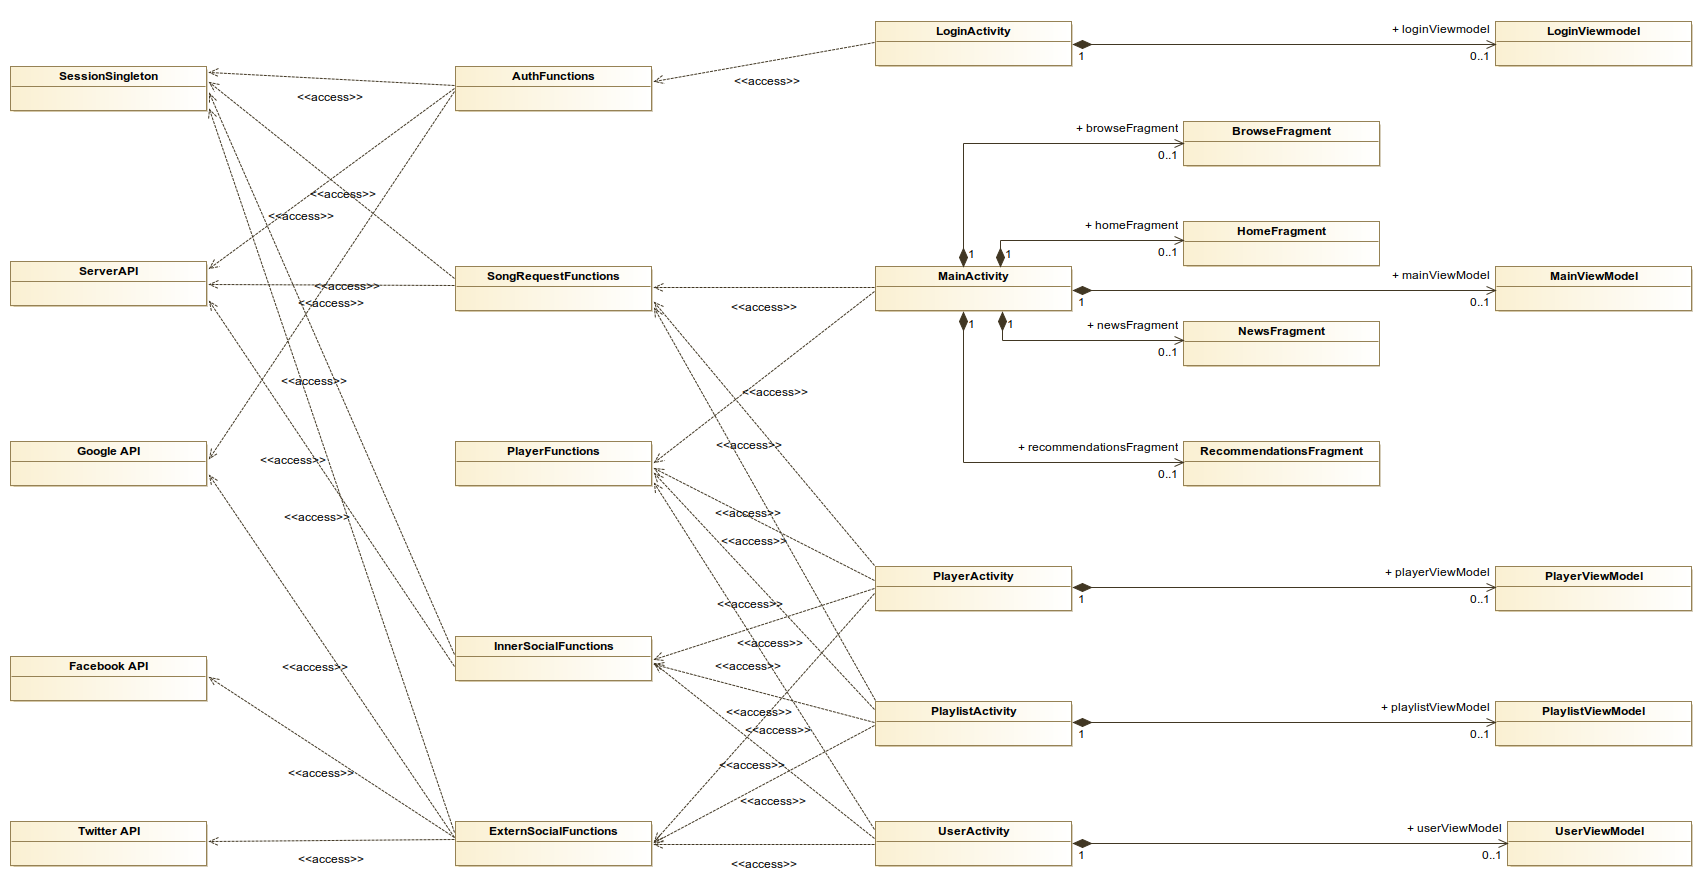
\includegraphics[width=\linewidth]{Figures/android-class.png}\\

\textbf{Diagrama de Gantt de la aplicaci\'on Android}\\
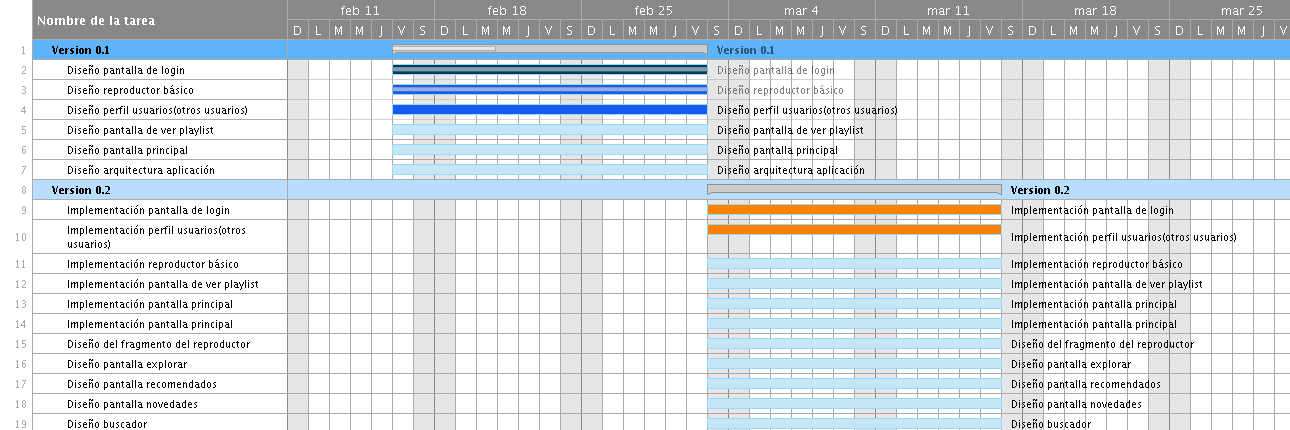
\includegraphics[width=\linewidth]{Figures/gantt-1.png}\\
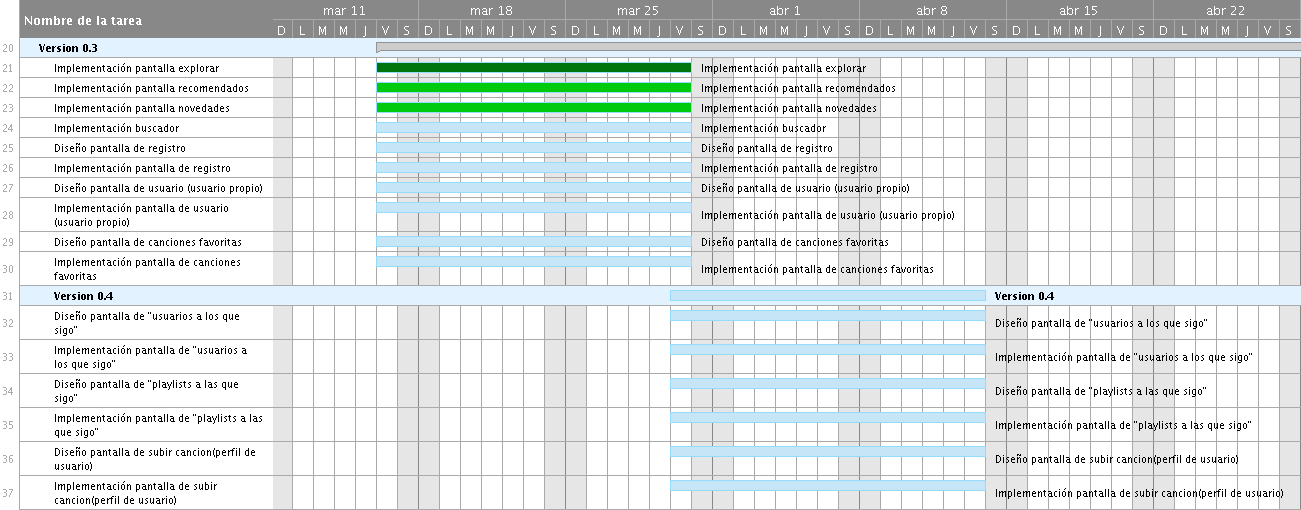
\includegraphics[width=\linewidth]{Figures/gantt-2.png}\\
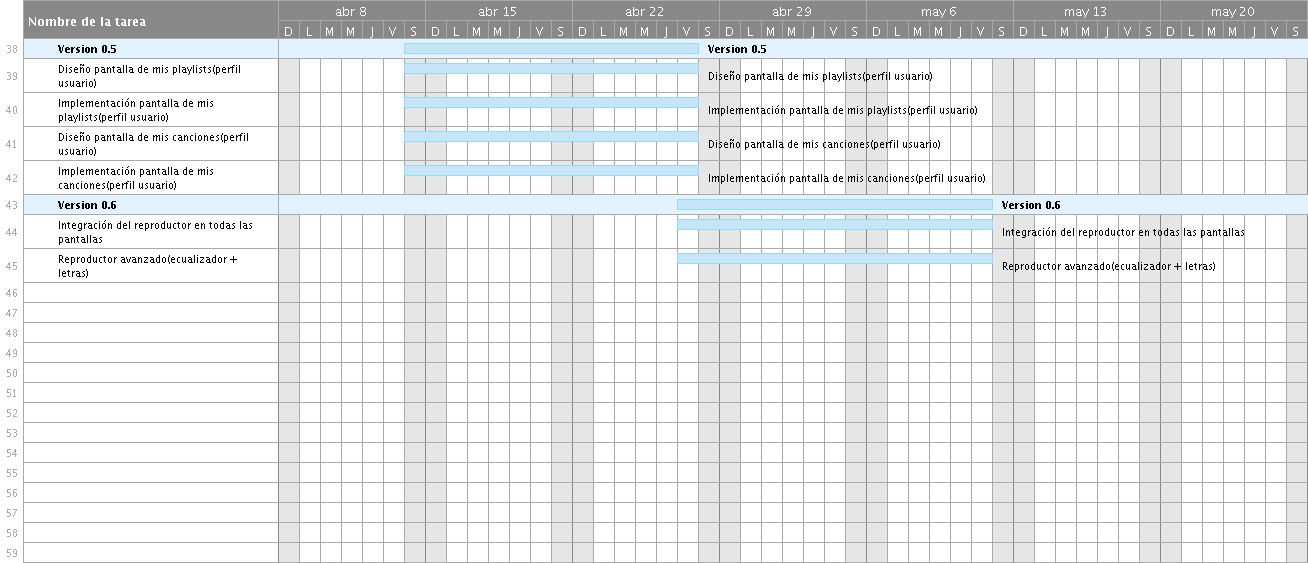
\includegraphics[width=\linewidth]{Figures/gantt-3.png}\\

\textbf{Versiones de la aplicaci\'on Android}

Versi\'on 0.1 (3 marzo)
Diseño pantalla de login
Diseño reproductor b\'asico
Diseño perfil usuarios(otros usuarios)
Diseño pantalla de ver playlist
Diseño pantalla principal (Aparecer\'an recomendaciones, novedades de artistas o playlists a las que se est\'e suscrito y canciones,playlists o artistas populares).
Diseño arquitectura aplicaci\'on

Versi\'on 0.2 (17 marzo)
Implementaci\'on pantalla de login
Implementaci\'on perfil usuarios(otros usuarios)
Implementaci\'on reproductor b\'asico
Implementaci\'on pantalla de ver playlist
Implementaci\'on pantalla principal (Aparecer\'an recomendaciones, novedades de artistas o playlists a las que se est\'e suscrito y canciones,playlists o artistas populares).
Diseño del fragmento del reproductor que aparecer\'a cuando se est\'a escuchando m\'usica en una pantalla que no es la pantalla de reproductor.
Diseño pantalla explorar (pantalla en la que aparecen todos los generos, artistas del momento y recomendaciones basadas en la ubicaci\'on).
Diseño pantalla recomendados
Diseño pantalla novedades
Diseño buscador

Versi\'on 0.3 (31 marzo)
Implementaci\'on pantalla explorar (pantalla en la que aparecen todos los generos, artistas del momento y recomendaciones basadas en la ubicaci\'on).
Implementaci\'on pantalla recomendados
Implementaci\'on pantalla novedades
Implementaci\'on buscador
Diseño pantalla de registro
Implementaci\'on pantalla de registro
Diseño pantalla de usuario (usuario propio)
Implementaci\'on pantalla de usuario (usuario propio)
Diseño pantalla de canciones favoritas
Implementaci\'on pantalla de canciones favoritas

Versi\'on 0.4 (14 abril)
Diseño pantalla de "usuarios a los que sigo"
Implementaci\'on pantalla de "usuarios a los que sigo"
Diseño pantalla de "playlists a las que sigo"
Implementaci\'on pantalla de "playlists a las que sigo"
Diseño pantalla de subir cancion(perfil de usuario)
Implementaci\'on pantalla de subir cancion(perfil de usuario)

Versi\'on 0.5 (28 abril)
Diseño pantalla de mis playlists(perfil usuario)
Implementaci\'on pantalla de mis playlists(perfil usuario)
Diseño pantalla de mis canciones(perfil usuario)
Implementaci\'on pantalla de mis canciones(perfil usuario)

Versi\'on 0.6 (\'ultima) (12 mayo)
Integraci\'on del reproductor en todas las pantallas
Reproductor avanzado(ecualizador + letras)


%% Section 4

\section{An\'alisis y dise\~no del sistema} % Main chapter title

\subsection{An\'alisis de requisitos}
\subsubsection{Sistema}
\textbf{Requisitos no funcionales}
\begin{enumerate}
	\item El sistema tendr\'a una versi\'on para Android y otra para Web.
	\item El sistema soporta los ficheros MP3, WAV, OGG.
	\item Existe un servidor para el almacenamiento de canciones.
	\item La aplicaci\'on movil soportar\'a Android 5.0 y la Web la \'ultima versi\'on de Firefox y Chrome.
\end{enumerate}



\subsubsection{Backend}
\textbf{Requisitos funcionales}
\begin{enumerate}

	\item El sistema se compone de Usuarios, Canciones y Listas de reproducci\'on.
	\item El sistema permite 3 tipos de usuarios:
	\begin{itemize}
		\item Usuario registrado (usuario que est\'e registrado en el sistema)
		\item Usuario no registrado (que es el cual el sistema no puede identificar con ninguna cuenta)
		\item Usuario administrador (aquel que es como un usuario registrado pero unos privilegios especiales, como es verificar cuentas)
	\end{itemize}
	\item Una canci\'on se compone de un t\'itulo, un audio, la transcripci\'on de dicho audio, el pa\'is de la canci\'on, cu\'antos me gusta tiene y el n\'umero de reproducciones.
	\item Una lista de reproducci\'on o categor\'ia es una lista de canciones generadas por el sistema agrupadas por g\'enero, \'exito, pa\'is, situaci\'on para la que es propicia o generada por el usuario.
	\item Un usuario registrado se compone de un nombre, un nick \'unico (es decir, que dos usuarios no pueden tener el mismo nick), un correo electr\'onico, una contrase\~na para acceder a la aplicaci\'on, la fecha de nacimiento, una biograf\'ia, una foto de perfil, qu\'e canciones ha reproducido, cu\'antos me gusta han recibido las canciones que ha subido, cu\'antos me gusta ha dado, sus canciones, el pa\'is y las redes sociales que quiera a\~nadir de forma opcional (Twitter, Facebook e Instagram).
	
	\item El sistema permite obtener todos los datos de una canci\'on.
	
	
	\item El sistema permite que los usuarios se registren en el sistema.
	\item El sistema permite que los usuarios de identifiquen tanto con usuario y contraseña as\'i como con una cuenta de Google.
	\item El sistema permite que los usuarios registrado registren nuevas canciones en el sistema.
	
	\item El sistema permite que los usuarios registrados creen y borren listas de reproducci\'on formadas por canciones que pueden ser o no del propio usuario, las cuales ser\'an p\'ublicas.
	\item El sistema permite que los usuarios registrados a\~nadan una canci\'on a una lista de reproducci\'on que haya creado \'el mismo.
	\item El sistema permite obtener todas las canciones de una lista de reproducci\'on.

	\item El sistema permite que los usuarios registrados tengan una lista de canciones favoritas, la cual ser\'a privada.
	\item El sistema permite que los usuarios registrados añadan o eliminen canciones de favoritos.
	\item El sistema permite que los usuarios registrados obtengan la lista de sus canciones favoritas.
	\item El sistema permite obtener las letras de una canci\'on.
	
	\item El sistema permite obtener recomendaciones (canciones, listas de reproducci\'on y usuarios), canciones m\'as populares, novedades sobre los usuarios o listas de reproducci\'on que un usuario sigue. 
	
	\item El sistema permite que los usuarios registrados modifiquen su nombre, su correo electr\'onico, su contrase\~na, su fecha de nacimiento, su biograf\'ia, su foto de perfil, su pa\'is y sus redes sociales.
	\item El sistema permite que los usuarios registrados sigan a una lista de reproducci\'on.
	\item El sistema permite buscar canciones mediante palabras clave (t\'itulo), g\'enero, pa\'is, me gusta, reproducciones o una combinaci\'on de varios.
	\item El sistema permite ver las canciones m\'as populares de un pa\'is.
	\item El sistema permite ver las canciones m\'as populares del pa\'is de un usuario.
	
	\item El sistema permite buscar artistas mediante palabras clave (nick, nombre y biograf\'ia), pa\'is o una combinaci\'on de varios.
	\item El sistema permite buscar listas de reproducci\'on mediante palabras clave (t\'itulo), canciones de la lista, tipo de orden de la lista o una combinaci\'on de varios.
	
	\item Las b\'usquedas por palabr\'as clave deber\'an contener al menos una palabra y, si contiene s\'olo una palabra, que sea de longitud mayor o igual a 3 caracteres.

\end{enumerate}

\textbf{Requisitos no funcionales}
\begin{enumerate}
	\item El nick de un usuario estar\'a compuesto por entre 4 y 32 caracteres.\\
	
\end{enumerate}

\subsubsection{Android}

\textbf{Requisitos funcionales}
\begin{enumerate}
	\item El sistema permite un solo tipo de usuario, y es el usuario registrado (usuario que est\'e registrado en el sistema).
	\item El sistema permite que los usuarios de identifiquen tanto con usuario y contraseña as\'i como con una cuenta de Google.
	\item  El sistema permite que los usuarios suban canciones a la aplicaci\'on
	\item  El sistema permite que los usuarios se registren en la aplicaci\'on.
	\item  El sistema permite a los usuarios tener una lista de canciones favoritas, la cual ser\'a privada.
	\item  El sistema permite añadir a favorito una canci\'on que se est\'a escuchando.
	\item  El sistema permite desde cualquier pantalla escuchar canciones y ver los controles b\'asicos de canciones (play, pause y pasar canci\'on)
	\item  El sistema permite desde una pantalla espec\'ifica acceder a m\'as controles sobre las canciones.
	\begin{itemize}
		\item  Desde la pantalla espec\'ifica el sistema permite avanzar o retroceder en la canci\'on a un momento exacto de esta.
		\item  Desde la pantalla espec\'ifica el sistema permite ver la letra de la canci\'on din\'amica (va al ritmo de la canci\'on) en el caso que la posea.
		\item  Desde la pantalla espec\'ifica el sistema permite ver la onda de sonido de la canci\'on.
		\item  Desde la pantalla espec\'ifica el sistema permite cambiar el orden de muestra de las canciones (aleatorio o lineal).
	\end{itemize}
	
	\item  El sistema posee una pantalla principal en la que se mostrar\'an recomendaciones (canciones, listas de reproducci\'on y usuarios), novedades sobre los usuarios y listas de reproducci\'on seguidos y canciones m\'as populares. 
	\item  El sistema posee una pantalla de usuario (otros usuarios) en la que se puede ver su informaci\'on, canciones, listas de reproducci\'on creadas, su n\'umero de seguidores, la opci\'on de seguirlo as\'i como un enlace a sus redes sociales.
	\item  El sistema posee una pantalla de usuario (usuario propio) en la que se puede ver las canciones del propio usuario y sus listas de reproducci\'on creadas, as\'i como añadir m\'as canciones, listas de reproducci\'on o eliminar alguna de las dos.
	
	\item  El sistema permite crear listas de reproducci\'on formadas por canciones de las que puedes ser autor o no, las cuales ser\'an publicas.
	\item  El sistema permite modificar los datos de usuario una vez creado.
	\item  El sistema posee una pantalla espec\'ifica en la que se puede ver las canciones que posee una lista de reproducci\'on as\'i como seguirla.
	\item  El sistema permite buscar las canciones m\'as populares de un g\'enero.
	\item  El sistema permite ver las canciones m\'as populares en el pa\'is desde el que se conecta el dispositivo.
	\item  El sistema permite buscar canciones, artistas y listas de reproducci\'on por su nombre mediante un buscador.
\end{enumerate}

\textbf{Requisitos funcionales}
\begin{enumerate}
	\item El sistema posee una pantalla principal en la que se mostrar\'an recomendaciones (canciones, listas de reproducci\'on y usuarios), novedades sobre los usuarios y listas de reproducci\'on seguidos y canciones m\'as populares. 
	\item El sistema posee una pantalla de usuario (otros usuarios) en la que se puede ver su informaci\'on, canciones, listas de reproducci\'on creadas, su n\'umero de seguidores, la opci\'on de seguirlo as\'i como un enlace a sus redes sociales.
	\item El sistema posee una pantalla de usuario (usuario propio) en la que se puede ver las canciones del propio usuario y sus listas de reproducci\'on creadas, as\'i como añadir m\'as canciones, listas de reproducci\'on o eliminar alguna de las dos.
\end{enumerate}

\subsubsection{Web}
	
\textbf{Requisitos funcionales}
\begin{enumerate}
	\item El sistema permite registrarse mediante usuario o a trav\'es de Google.
	\item Verificaci\'on de cuenta. Esto supone un indicador gr\'afico en el perfil de usuario que anteriormente a verificado su identidad. La finalidad es garantizar la verdadera identidad del usuario.
	\item La reproducci\'on actual de un usuario se sincroniza en todos los dispositivos.
	
	\item Existen 3 perfiles de usuarios: registrados, no registrados y administrador.
	\begin{enumerate}
		\item Registrados
		\begin{enumerate}
			\item Los usuarios no registrados pueden acceder a la p\'agina principal, p\'aginas de los diferentes usuarios, p\'aginas de canciones ademas de poder realizar b\'usquedas.
			\item Los usuarios no registrados pueden reproducir canciones de usuarios o de listas de reproducci\'on p\'ublicas.
			
		\end{enumerate}
		\item Registrados
		\begin{enumerate}
			\item Los usuarios registrados pueden realizar todas las funcionalidades de un usuario no registrado.
			\item El sistema permite a los usuarios registrados identificarse.
			\item El sistema permite a los usuarios registrados modificar su informaci\'on personal.
			\item El sistema permite a los usuarios registrados subir canciones.
			\item El sistema permite administrar una lista de reproducci\'on privada de favoritos.
			\item El sistema permite añadir cualquier canci\'on a favoritos.
			\item El sistema permite crear listas de reproducci\'on p\'ublicas
			\item El sistema permite añadir cualquier canci\'on a una lista de reproducci\'on previamente creada por el usuario.
			\item El sistema permite eliminar una canci\'on de sus listas de reproducci\'on o de la lista favoritos.	
			\item El sistema permite seguir/ dejar de seguir a un usuario.
			\item El sistema permite seguir/ dejar de seguir a una lista de reproducci\'on.
			\item El sistema permite modificar sus enlaces a redes sociales.
			\item (RNF) La pantalla principal de un usuario registrado contiene recomendaciones de artistas, listas o usuarios en base a sus gusto y novedades de sus artistas/listas seguidos.
		\end{enumerate}
		\item Administrador
		\begin{enumerate}
			\item El usuario administrador se identifica en la aplicaci\'on con un usuarios y contraseña predefinidos.
			\item El sistema permite al usuario administrador puede verificar la identidad de un usuario.
			\item El sistema permite al usuario administrador modificar la informaci\'on de un usuario, canci\'on o playlist.
			\item (RNF) La pantalla de administrador incluye un buscador para la b\'usqueda de un usuario, lista o canci\'on y una lista con el resultado de la b\'usqueda.
			\item (RNF) Cada canci\'on, lista o usuario tiene una pantalla de administrador desde donde el sistema permite al administrador la modificaci\'on.
			
		\end{enumerate}
	\end{enumerate}
\end{enumerate}
	
\textbf{Requisitos no funcionales}
\begin{enumerate}
	\item El sistema tiene una pantalla principal donde se mostraran novedades de artiastas y canciones y canciones mas populares.
	\item El sistema tiene una pantalla de ususario p\'ublica para todo el mundo donde aparece su informaci\'on, canciones, listas de reproducci\'on p\'ublicas, n\'umero de seguidores y enlaces a sus redes sociales
	\item El sistema cuenta en todas las pantallas con un reproductor de audio que incluye informaci\'on sobre la canci\'on que se esta reproduciendo y las opciones de avanzar, retroceder a un momento de la canci\'on; avanzar o retroceder a la siguiente o anterior canci\'on si se esta reproduciendo una lista; parar la reproducci\'on y cambiar el orden de reproducci\'on a aleatorio.
	\item El sistema tiene en todas las pantallas un buscador para realizar una b\'usqueda de canciones, listas y usuarios.
	\item El sistema tiene una pantalla para cada canci\'on donde se puede ver la  informaci\'on de la canci\'on, la onda de sonido y si tuviese las letras de \item forma din\'amica si se estuviese reproduciendo.
	\item El sistema tiene una pantalla para identificarse/ registrarse.
\end{enumerate}

\subsection{Dise\~no del sistema}
\begin{itemize}
	\item Diagramas arquitecturales (de m\'odulos, de componentes y conectores, de distribuci\'on), patrones de dise\~no y estilos arquitecturales que se aplicar\'an. Las interfaces (de m\'odulos y de componentes) son especialmente importantes. Tambi\'en lo son los protocolos de comunicaci\'on entre componentes.
	\item Tecnolog\'ias elegidas (lenguajes de programaci\'on, componentes que se integrar\'an, API web externas con las que se conectar\'a etc.).
	\item Otros aspectos t\'ecnicos de inter\'es (p.ej. si hay base de datos si va a ser SQL o NoSQL, si hay una API Web va a ser RESTful o no, si algunas de las operaciones van a ser as\'incronas o no, si va a ser una aplicaci\'on m\'ovil o de escritorio ser\'a nativa o se van a usar tecnolog\'ias web, c\'omo se van a considerar los requisitos de seguridad o de prestaciones, c\'omo y d\'onde se har\'an las instalaciones y despliegues etc.)
\end{itemize}

Hay que justificar todas las decisiones de dise\~no. Esto exige contestar a dos preguntas sobre cada decisi\'on: ¿qu\'e alternativas se barajaron? y ¿por qu\'e se eligi\'o una y no las otras?


%% Section 5

%\section{Memoria del proyecto} % Main chapter title
%
%\label{Chapter5} % Change X to a consecutive number; for referencing this chapter elsewhere, use \ref{ChapterX}
%
%
%ESTE CAP\'iTULO NO SE RELLENA EN LA PRIMERA ENTREGA
%En este cap\'itulo se describir\'a c\'omo se ha llevado a cabo el proyecto, qu\'e cambios se han hecho respecto a la versi\'on inicial, imprevistos surgidos, etc.
%\subsection{Inicio del proyecto}
%Describir c\'omo transcurri\'o esta fase del proyecto, especialmente los resultados de llevar a cabo los procesos descritos en la secci\'on Procesos de inicio del proyecto.
%\subsection{Ejecuci\'on y control del proyecto}
%Describir c\'omo transcurri\'o esta fase del proyecto, especialmente los resultados de llevar a cabo los procesos descritos en la secci\'on Procesos de ejecuci\'on y control del proyecto y en la secci\'on Procesos t\'ecnicos. No olvidar:
%\begin{itemize}
%	\item C\'omo se ha realizado el reparto de trabajo entre miembros del equipo. C\'omo ha transcurrido la comunicaci\'on interna.
%	\item C\'omo se ha medido el progreso del proyecto. C\'omo se sab\'ia el trabajo realizado, el trabajo pendiente y lo que estaba haciendo cada persona.
%	\item Los ajustes realizados cuando se detectaron divergencias frente al calendario inicial (ajustes en el trabajo y/o ajustes en el calendario). Si se han identificado las causas de estas divergencias, explicarlas.
%	\item Adecuaci\'on de las herramientas y tecnolog\'ias empleadas. Si ha habido que cambiar alguna decisi\'on de dise\~no o de tecnolog\'ia, y por qu\'e.
%	\item Funcionamiento de los procesos de control de versiones del c\'odigo, construcci\'on y despliegue. ¿Ha habido problemas con las integraciones? ¿Problemas con los despliegues? ¿Se han perdido cosas por errores humanos? ¿C\'omo se han abordado estas tareas?
%	\item Pruebas del software. ¿Se han podido cumplir las ideas que se ten\'ian al respecto?
%\end{itemize}
%
%\subsection{Cierre del proyecto}
%Al menos:
%\begin{itemize}
%	\item Comparar las estimaciones iniciales (tama\~no, esfuerzos, costes) con los resultados finales, analizar los resultados y tratar de expresar algunas lecciones aprendidas.
%	\item Lecciones aprendidas sobre herramientas y tecnolog\'ias.
%	\item Recopilar los esfuerzos dedicados al proyecto por cada uno de los participantes: horas trabajadas y actividades realizadas por cada persona.
%\end{itemize}

%% Section 6

%\section{Conclusiones} % Main chapter title
%
%
%ESTE CAP\'iTULO SOLO SE RELLENA EN LA ENTREGA FINAL
%Adem\'as de conclusiones personales (razonadas) sobre el transcurso del proyecto realizado, es importante plantear ideas para mejorar los procesos llevados a cabo: si hubiera que iniciar un nuevo proyecto inmediatamente usando una metodolog\'ia de gesti\'on basada en procesos, ¿qu\'e cambios har\'iais respecto a los procesos que hab\'eis seguido durante este proyecto?  ¿Qu\'e cosas est\'a claro que har\'iais de otra forma? ¿Qu\'e cosas seguir\'iais haciendo m\'as o menos igual?


\end{document}